%%%%%%%%%%%%%%%%%%%%%%%%%%%%%%%%%%%%%%%%%
% Stylish Article
% LaTeX Template
% Version 2.1 (1/10/15)
%
% This template has been downloaded from:
% http://www.LaTeXTemplates.com
%
% Original author:
% Mathias Legrand (legrand.mathias@gmail.com) 
% With extensive modifications by:
% Vel (vel@latextemplates.com)
% Final ACS by:
% Juan Barbosa
% License:
% CC BY-NC-SA 3.0 (http://creativecommons.org/licenses/by-nc-sa/3.0/)
%
%%%%%%%%%%%%%%%%%%%%%%%%%%%%%%%%%%%%%%%%%
\documentclass[fleqn,10pt]{SelfArx}
%\usepackage[superscript]{cite}
\usepackage{wrapfig}
\usepackage{subcaption}
\usepackage[numbers, super]{natbib}
%----------------------------------------------------------------------------------------
%	ARTICLE INFORMATION
%----------------------------------------------------------------------------------------

\JournalInfo{Laboratorio Org\'anica 3, No. 3, 09/09/2017} % Journal information
\Archive{ }

\PaperTitle{Reacci\'on de Ozon\'olisis} %
%\Keywords{Keyword1 --- Keyword2 --- Keyword3} % Keywords - if you don't want any simply remove all the text between the curly brackets
%\newcommand{\keywordname}{Keywords} % Defines the keywords heading name

%----------------------------------------------------------------------------------------
%	ABSTRACT
%----------------------------------------------------------------------------------------

\Abstract{
\begin{wrapfigure}{r}{0.45\textwidth}
	\centering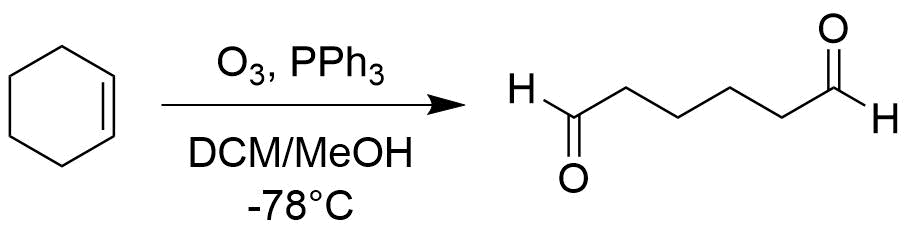
\includegraphics[width=0.9\linewidth]{structures/overall.png}
\end{wrapfigure}

La preparaci\'on de adipaldehído fue realizada a partir de ciclohexeno, en presencia de ozono y trifenilfosfina. El tiempo de reacci\'on fue inferior a los 10 minutos, el producto fue purificado en columna obteniendose un porcentaje de recuperaci\'on de 72 \% y un rendimiento de 53 \%. El producto fue caracterizado usando t\'ecnicas espectrosc\'opicas como $^1$HRMN y $^{13}$CRMN.
}

%----------------------------------------------------------------------------------------

\begin{document}

\flushbottom % Makes all text pages the same height

\maketitle % Print the title and abstract box

%\tableofcontents % Print the contents section

\thispagestyle{empty} % Removes page numbering from the first page
\renewcommand{\tablename}{Tabla} 


%----------------------------------------------------------------------------------------
%	ARTICLE CONTENTS
%----------------------------------------------------------------------------------------

\section*{Introducci\'on} % The \section*{} command stops section numbering
%------------------------------------------------
La ozon\'olisis representa una importante reacci\'on oxidativa en la qu\'imica org\'anica. Como todas las reacciones de oxidaci\'on tienen una especial importancia en la qu\'imica, ya que permiten convertir grupos funcionales y preparar compuestos complejos a partir de reactivos simples. Si bien la definici\'on qu\'imica de oxidaci\'on involucra una transferencia de electrones en la cual la mol\'ecula o \'atomo oxidado pierde electrones, en la qu\'imica org\'anica la oxidaci\'on muchas veces implica el aumento de enlaces carbono-ox\'igeno en una mol\'ecula, aunque no es la \'unica forma de oxidaci\'on \cite{Gilbert2010}.

La mayor\'ia de las reacciones de los alquenos, transforman el enlace $\pi$ en un enlace $\sigma$ aprovechando la riqueza electr\'onica de los enlaces dobles. Los alquenos al igual que otros grupos funcionales presentan principalmente tres tipos de reacciones: adici\'on, eliminaci\'on y sustituci\'on, sin embargo tambi\'en existe la posibilidad de reacciones de ruptura: una reacci\'on donde el enlace $\pi$ se rompe y el alqueno se transforma en dos mol\'eulas m\'as peque\~nas. La reacci\'on de ozon\'olisis adem\'as de generar dos nuevos enlaces carbono-ox\'igeno, da lugar a la degradaci\'on de la mol\'ecula inicial, esto impl\'ica que se clasifica como una reacci\'on de oxidaci\'on y ruptura \cite{Wade2013}\cite{Morrison2002}.
\begin{scheme}[h]
	\centering
	\caption{Reacci\'on de ozonolisis \cite{Wade2013}.}
	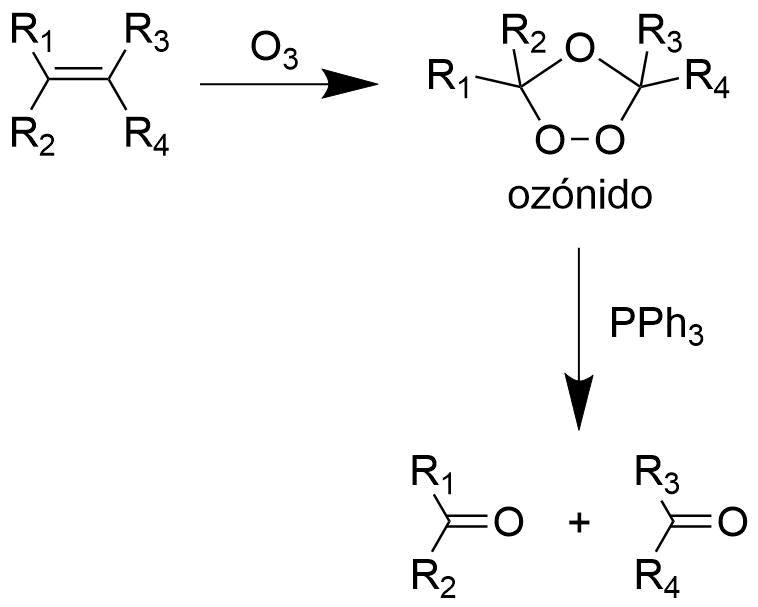
\includegraphics[width=0.7\linewidth]{structures/ozonolisis.png}
\end{scheme}

La reacci\'on de ozon\'olisis recibe su nombre debido a que la oxidaci\'on se lleva a cabo con ozono, el cual se adiciona sobre el doble enlace para formar un oz\'onido, seguido de la ruptura del alqueno \cite{Morrison2002}. El ozono es una mol\'ecula altamente reactiva, presenta 142 kJ/mol m\'as de energ\'ia comparada con el ox\'igeno molecular, parte de su reactividad obdece a la densidad de carga positiva sobre el ox\'igeno central \cite{Wade2013}. Uno de los usos m\'as comunes de la ozon\'olisis es la determinaci\'on de la ubicaci\'on de una insaturaci\'on en los alquenos.
\begin{figure}[h]
	\centering
	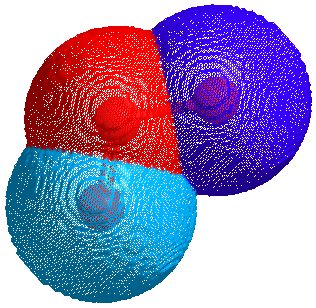
\includegraphics[width=0.4\linewidth]{structures/ozone.png}
	\caption{Densidades de carga en el ozono. De izquierda a derecha: -0.80$e$, 1.10$e$, -0.30$e$. Valores basados en el modelo de H\"uckel \cite{PerkinElmer}.}
\end{figure}

El ozono es particularmente peligroso por su capacidad oxidativa, en el cuerpo humano es capaz de irritar los pulmones y generar cansancio. Adem\'as puede incrementar la sensibilidad de una persona a los al\'ergenos, esto debido a que el ozono oxida los enlaces $\pi$ de los \'acidos grasos que forman la superficie de las membranas celulares\cite{Wade2013}.
\newpage
\section{Resultados y Discusi\'on}
En el espectro $^1$HRMN obtenido del producto final se pueden observar distintas señales, dentro de las cuales destacan los desplazamientos de la molécula que se buscaba obtener, el adipaldehído (\autoref{HRMN}). Esta molécula cuenta con seis carbonos distintos, pero al tener un plano de simetría, en el espectro se pueden observar únicamente tres picos propios de esta molécula: $\delta$ 9.79 \textbf{(a)}, 2.56 - 2.43 \textbf{(b)} y 1.69 - 1.66 \textbf{(c)}. Estos desplazamientos muestran excelente correspondencia con respecto a los valores reportados en la literatura\cite{Miller2017}. Los desplazamientos se explican con la presencia de los grupos carbonilo, en donde los protones más desplazados son aquellos que se encuentran enlazados directamente al carbonilo \textbf{(a)}. Esto se debe a que este grupo es fuertemente extractor de carga, y por lo tanto los protones ligados a ellos se verán altamente desprotegidos, por lo que en un espectro sus señales aparecen en campo bajo \textbf{(b)}. 
\begin{scheme}[h]
	\centering
	\caption{Protones del adipaldeh\'ido.}
	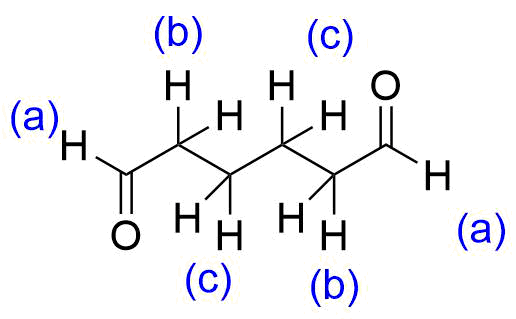
\includegraphics[width=0.5\linewidth]{structures/hidrogenos.png}
\end{scheme}

Los protones que se encuentran a dos enlaces de distancia de este grupo no se ven tan afectados por esto, y por lo tanto su señal aparece hacia campo más alto \textbf{(c)}. Los protones más alejados se encuentran más protegidos, y por lo tanto sus señales aparecen alrededor de 1.60, lo cual es campo alto. Esta misma tendencia se puede observar en los carbonos en el espectro $^{13}$CRMN. Además de las señales correspondientes al compuesto objetivo, también se observan distintas señales, las cuales corresponden a contaminación del producto con distintos compuestos, dentro de los cuales se puede observar trifenilfosfina, metanol, diclorometano y cloroformo.

Para no observar solvente en la muestra, es crucial remover el solvente una vez terminada la reacción. Como se mencionó anteriormente, remover la trifenilfosfina del producto final es complicado, ya que puede presentar una polaridad similar. Por lo tanto, es recomendable utilizar otro agente reductor, como \ce{Me2S}, aun cuando el tiempo de reacción sea mayor.

Los espectros de resonancia magn\'etica nuclear adem\'as de permitir elucidar el producto permiten describir la pureza del mismo. Lo anterior es posible si se identifican las se\~nales asociadas a las impurezas. Conociendo la relaci\'on entre las integrales de los hidr\'ogenos se obtiene la cantidad relativa de los mismos en la muestra, y conociendo la masa neta se determina la masa real del producto.
\begin{equation}
R_{(p, i)} = \left(\dfrac{n_H^{p}}{I_H^{(p)}}\right)\dfrac{I^{(i)}_H}{n_H^{(i)}}
\end{equation}
\pagebreak

Donde $R_{(p, i)}$ es la relaci\'on producto impureza, esto es el n\'umero de mol\'eculas de una impureza por cada mol\'ecula de producto. La concentraci\'on relativa del producto en la muestra se determina considerando la relaci\'on producto producto $R_{(p, p)} \equiv 1$ y el n\'umero total de mol\'eculas de los $N$ compuestos identificados en la muestra.
\begin{equation}\label{eq: concentracion}
C_{rel} = \dfrac{1}{\sum\limits_{j = 0}^{N} R_{(p, j)}}
\end{equation}

En el \autoref{tb: pureza} se muestran las impurezas identificadas, junto con su relaci\'on producto impureza y la concentraci\'on relativa. Usando la \autoref{eq: concentracion} se determina la concentraci\'on del producto en 73 \%. Sin embargo es necesario tener en cuenta que existen compuestos no identificados en el espectro, adem\'as que este m\'etodo no cuantifica compuestos que no contengan protones. Por esta raz\'on el valor de pureza no se puede determinar con seguridad y \'unicamente se puede acotar, la pureza m\'axima del producto es entonces 73 \%.
\begin{table}[h]
	\centering
	\caption{Impurezas identificadas}
	\begin{tabular}{ccccc}
		\hline
		\textbf{Compuesto} & $n_H$ & $I_H$ & $R_{(p, i)}$ & $C_{rel}$\\
		\hline
		\ce{CHCl3} & 1 & 0.18 &
		0.18 & 0.13\\
		\ce{PPh3} & 15 & 1.48 & 0.10 & 0.07\\
		\ce{CH2Cl2} & 2 & 0.16 &
		0.08 & 0.06\\
		\ce{CH3OH} & 4 & 0.08 & 0.02 & 0.01\\
		\hline
	\end{tabular}
	\label{tb: pureza}
\end{table}
\begin{scheme*}[h]
	\centering
	\caption{Mecanismo de reacci\'on propuesto.}
	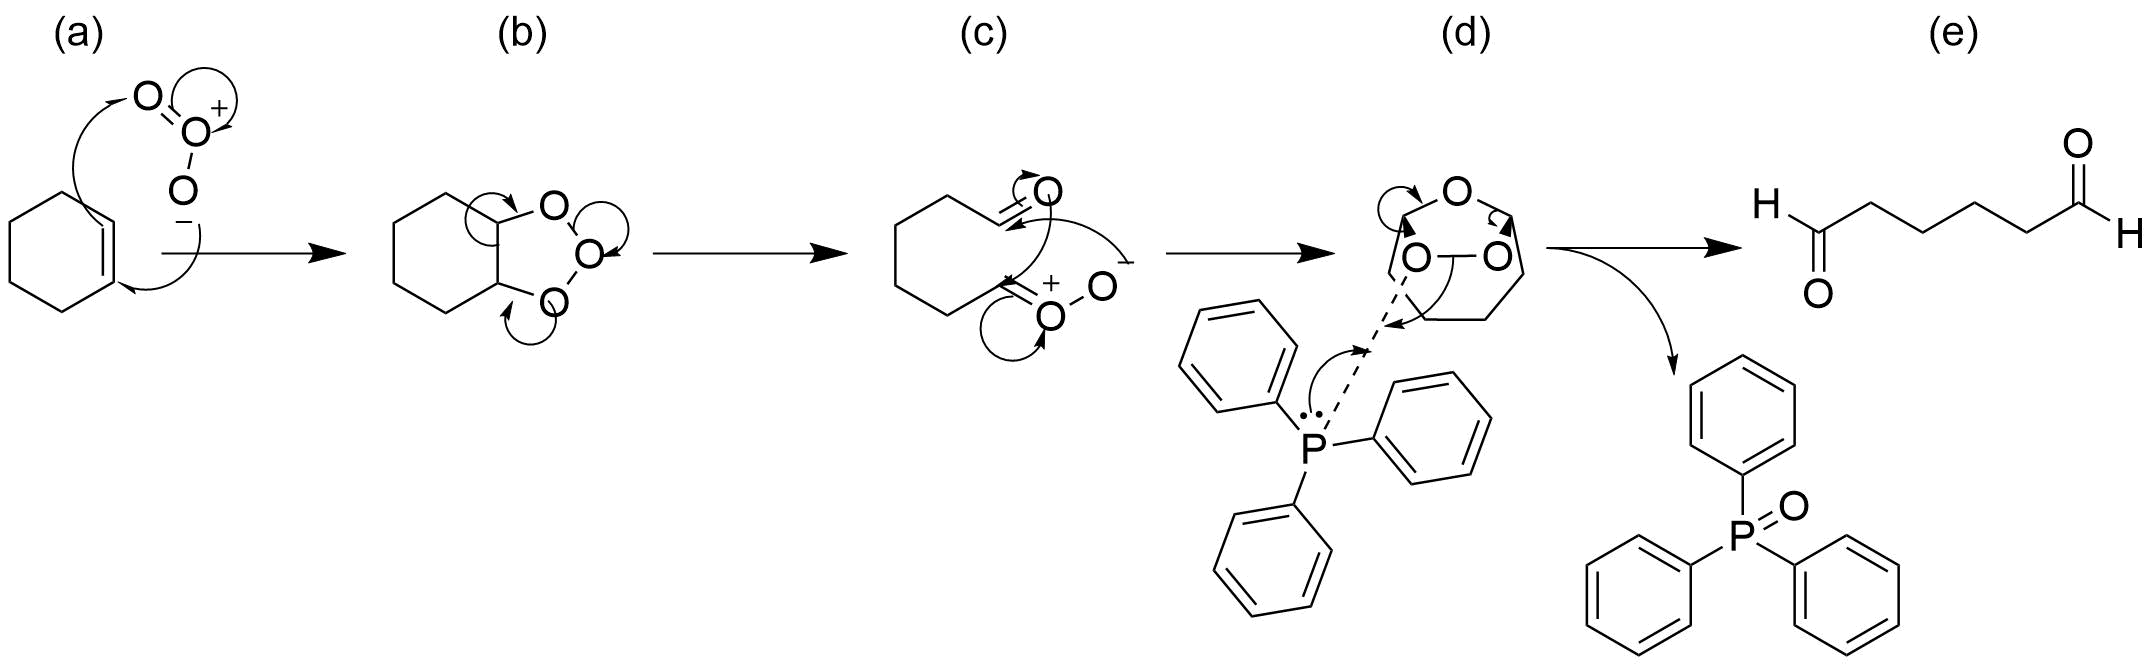
\includegraphics[width=0.9\linewidth]{structures/mecanismo.png}
	\label{sch: mecanismo}
\end{scheme*}

A partir de esto y teniendo en cuenta la masa neta obtenida, junto con el n\'umero de moles de ciclohexeno adicionado (2.43 mmol) se determina el rendimiento en 53 \%.

El rendimiento obtenido resulta considerablemente menor comparado con otros m\'etodos de preparaci\'on publicados en la literatura que alcanzan el 97 \%\cite{Liu2007} y 100 \%\cite{Daw2014}. Estos m\'etodos tienen en particular el uso de sistemas catal\'iticos con metales, evitando de esta forma los pel\'igros del manejo del ozono, el uso de uso de bajas temperaturas, y mejorando el control de la oxidaci\'on de los productos, alcanzando \'unicamente el aldeh\'ido o cetona y no el \'acido \cite{Daw2014}.

En la mayor\'ia de los casos las condiciones de oxidaci\'on son tan fuertes que los metales se usan como sales, nanopart\'iculas y \'oxidos, dado que los ligandos muchas veces se descomponen en estas condiciones. Sin embargo existen varios ligandos capaces de soportar tales condiciones, entre esos se encuentran los ligandos donores de nitr\'ogeno, los cuales presentan deslocalizaci\'on $\pi$, esto resulta particularmente importante porque incrementan la retrodonaci\'on metal ligando al aumentar el car\'acter $\sigma$ donor\cite{Daw2014}.

La obtención del adipaldehído a partir de ciclohexeno y ozono se realiza a través de un mecanismo de reacción en el cual primero se obtiene un intermediario ozónido y posteriormente, a través de un agente reductor, se obtienen el aldehído\cite{Carey2007} (\autoref{sch: mecanismo}). La obtención del primer intermediario se realiza a través de una serie de tres reacciones de cicloadición [2 + 3]\cite{Criegee1975}. En primer lugar, se realiza la adición del ozono al doble enlace, produciendo de esta manera un ozónido primario \textbf{(a)}. Posteriormente, este intermediario se descompone en un carbonilo y un óxido carbonílico \textbf{(b)}, el cual finalmente se adiciona sobre el carbonilo \textbf{(c)}, produciendo otro intermediario ozónido \textbf{(d)}\cite{Wade2013}. Posteriormente la trifenilfosfina act\'ua como agente reductor, dando lugar al dialdeh\'ido y al \'oxido de trifenilfosfina \textbf{(e)}.

La trifenilfosfina resulta ventajosa ya que presenta una gran actividad a temperaturas bajas, lo cual es apropiado debido a que esta reacción se realiza a temperaturas por debajo de 0 $^\circ$C. Esto significa que la reacción se realiza rápidamente de una manera conveniente\cite{Knowles1960}. Sin embargo, el uso de este reductor puede llegar a ser un inconveniente al momento de separar el aldehído obtenido de la fosfina, en especial si el producto presenta una polaridad similar a la trifenifosfina\cite{doi:10.1080/00397918608057738}. Para evitar esta complicación, se pueden utilizar agentes reductores alternos, como lo son el zinc, el dimetilsulfuro, fosfinas poliméricas, entre otras\cite{Wade2013}\cite{doi:10.1080/00397918608057738}. Sin embargo, hay que tener en cuenta que estas reacciones toman más tiempo, ya que estos agentes reductores no son tan activos a bajas temperaturas como la trifenilfosfina.

Un aspecto importante que se debe tener en cuenta al realizarse esta reacción es que es necesario el uso de solventes inertes, los cuales no contengan alcoholes. En presencia de alcoholes, el carbonilo producido por la descomposición del ozónido primario se ve atrapado en forma de $\alpha$-hidroperoxi éter\cite{Keaveney1967}, de la siguiente manera:
\begin{scheme}[h]
	\centering
	\caption{Reacci\'on en presencia de alcohol.}
	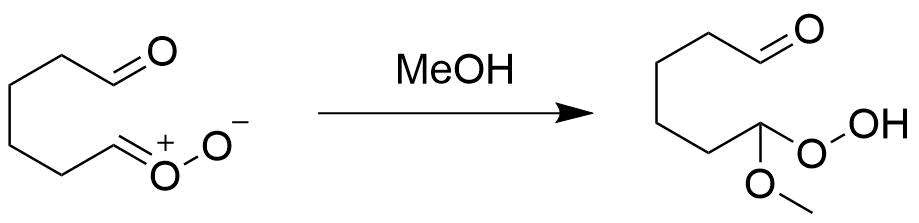
\includegraphics[width=0.7\linewidth]{structures/metanol.png}
\end{scheme}

Esto causa que no se pueda volver a formar el ozónido y continuar con la reacción de ozonólisis\cite{Carey2007}. Por lo tanto, si hay alcohol en el medio se producirán compuestos distintos al objetivo que pueden causar una disminución en el rendimiento. Debido a esto, se recomienda utilizar únicamente solventes que no tengan el grupo alcohol.

\newpage
\section{Conclusiones}
Se obtuvo adipaldehído mediante una reacción de ozonólisis del ciclohexeno, obteniendo un porcentaje de recuperación del 76 \% y un rendimiento del 53 \%. Se caracterizó mediante RMN de $^1$H y $^{13}$C, y se obtuvieron los picos esperados para el producto objetivo. La reacción se llevó acabo en un medio de alcohol, el cual reacciona con uno de los intermediarios de la reacción, lo cual pudo afectar el rendimiento obtenido. Otra complicación que se pudo observar es la presencia de trifenilfosfina y su dificultad para ser separado del compuesto, ya que puede presentar polaridades similares al producto. Se concluyó que las mejoras que se pueden realizar al procedimiento es eliminar el uso de metanol como solvente e únicamente utilizar diclorometano, adem\'as de un agente reductor diferente.

\section{Secci\'on experimental}
En un bal\'on de ozon\'olisis se mezclaron 2.43 mmol de ciclohexeno y 2.67 mmol de trifenilfosfina (\ce{PPh3}), en una soluci\'on de 16 mL de diclorometano y 4 mL de metanol. El bal\'on se enfri\'o en un vaso de Dewar a -78 $^\circ$C. Usando un generador de ozono a 30 vatios se burbuje\'o directamente el mismo hasta observar coloraci\'on azul en el bal\'on. Posteriormente se adiciona ox\'igeno gaseoso hasta revertir el color. La soluci\'on se calienta a temperatura ambiente por 4 horas. 

El producto se purifica en columna de s\'ilica usando una fase m\'ovil acetato de etilo : n-pentano (1:1). Las fracciones 6 a la 13 se concentran a presi\'on reducida, finalmente los remanentes de disolvente se evaporan usando cloroformo como solvente de arrastre a una temperatura de 47 $^\circ$C y 11 mBar de presi\'on.

\paragraph{Adipaldeh\'ido:}
$^1$H NMR (400 MHz, \ce{CDCl3}) $\delta$ 9.79 (t, 1H), 2.56 – 2.43 (m, J = 14.9, 4.9, 3.4 Hz, 2H), 1.69 – 1.66 (m, 2H).

$^{13}$C NMR (101 MHz, CDCl3) $\delta$ 201.97 (s), 43.61 (s), 21.73 (s).

%----------------------------------------------------------------------------------------
%	REFERENCE LIST
%----------------------------------------------------------------------------------------
\newpage
\phantomsection
\bibliography{informe}
\bibliographystyle{achemso}

%----------------------------------------------------------------------------------------
\newpage
\onecolumn
\section{Informaci\'on suplementaria}\label{sec: complementaria}
\begin{figure}[h]
	\centering
	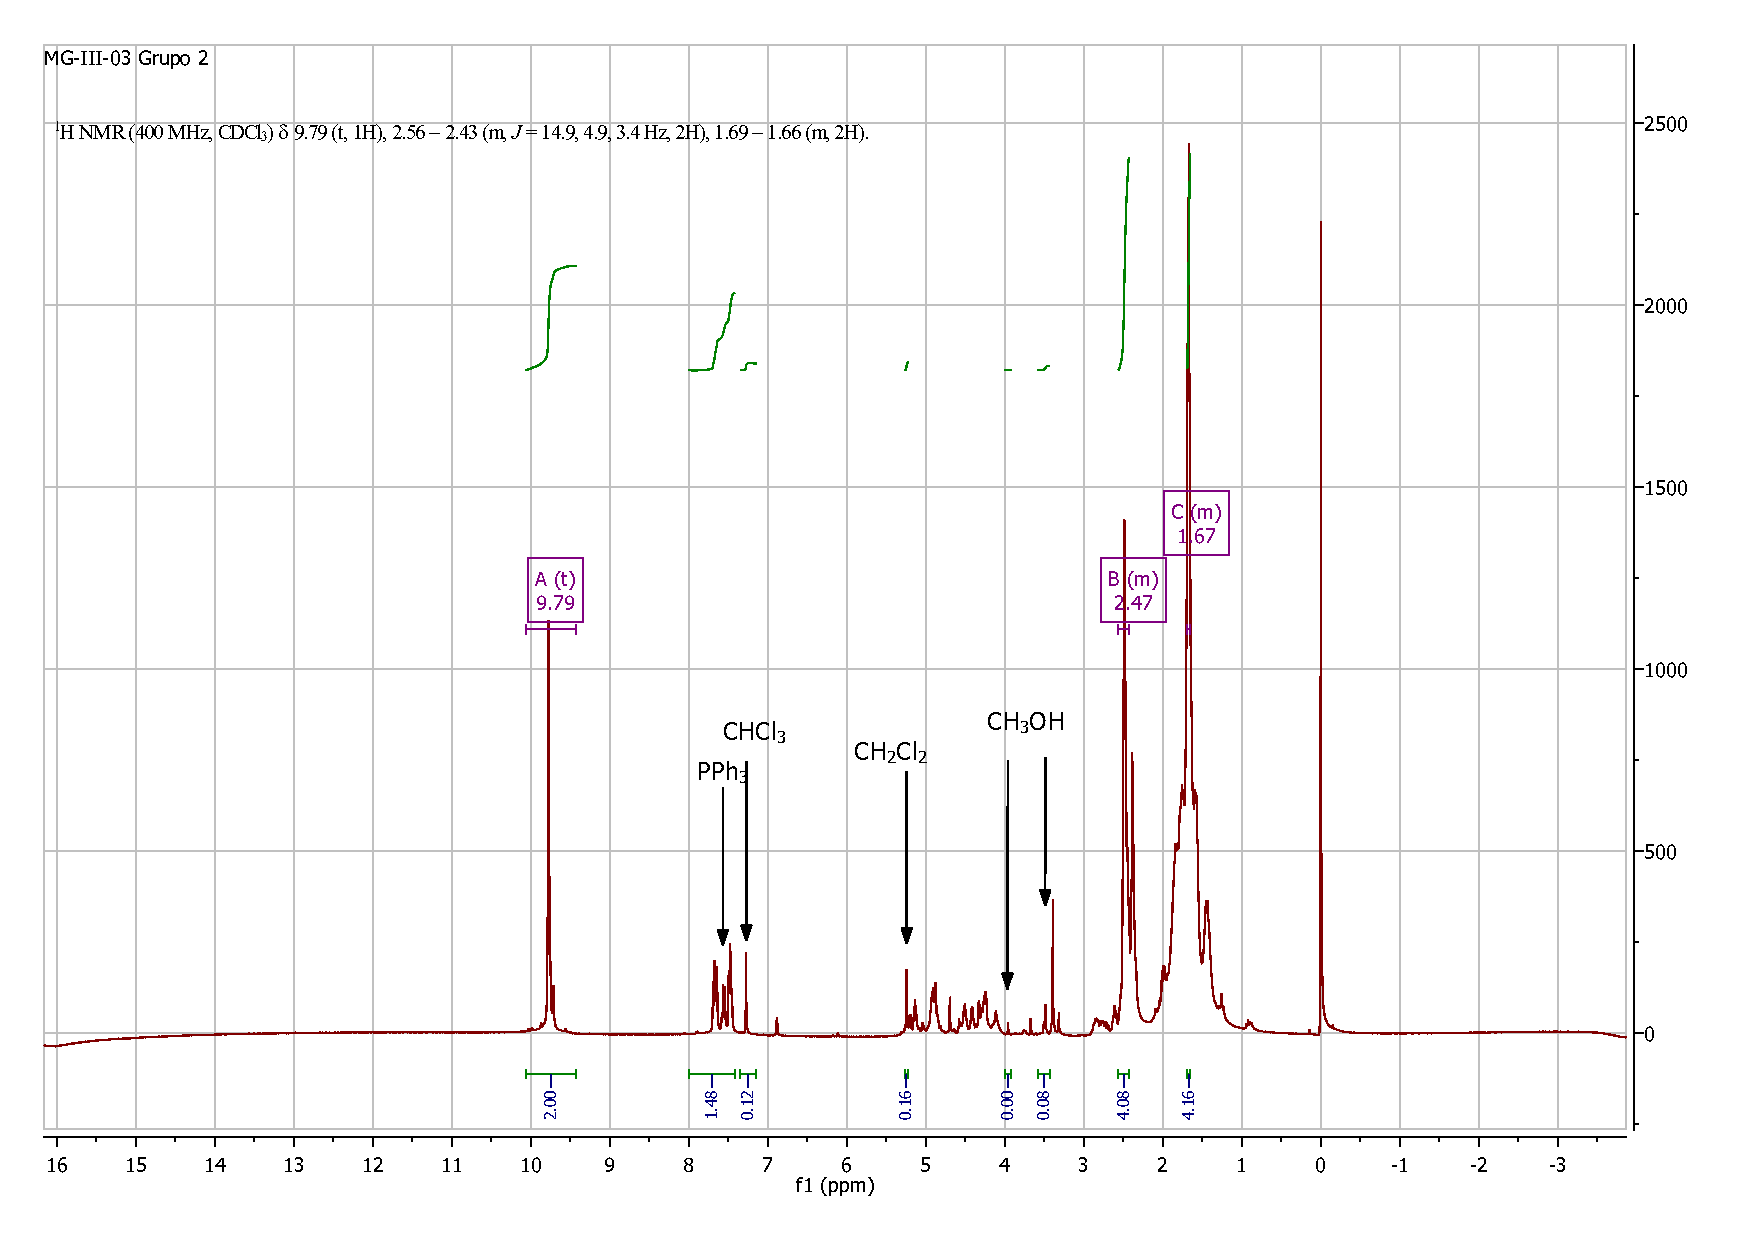
\includegraphics[width=0.5\textheight]{RMN/H.pdf}
	\caption{$^1$HRMN del producto purificado.}
	\label{HRMN}
\end{figure}
\begin{figure}[h]
	\centering
	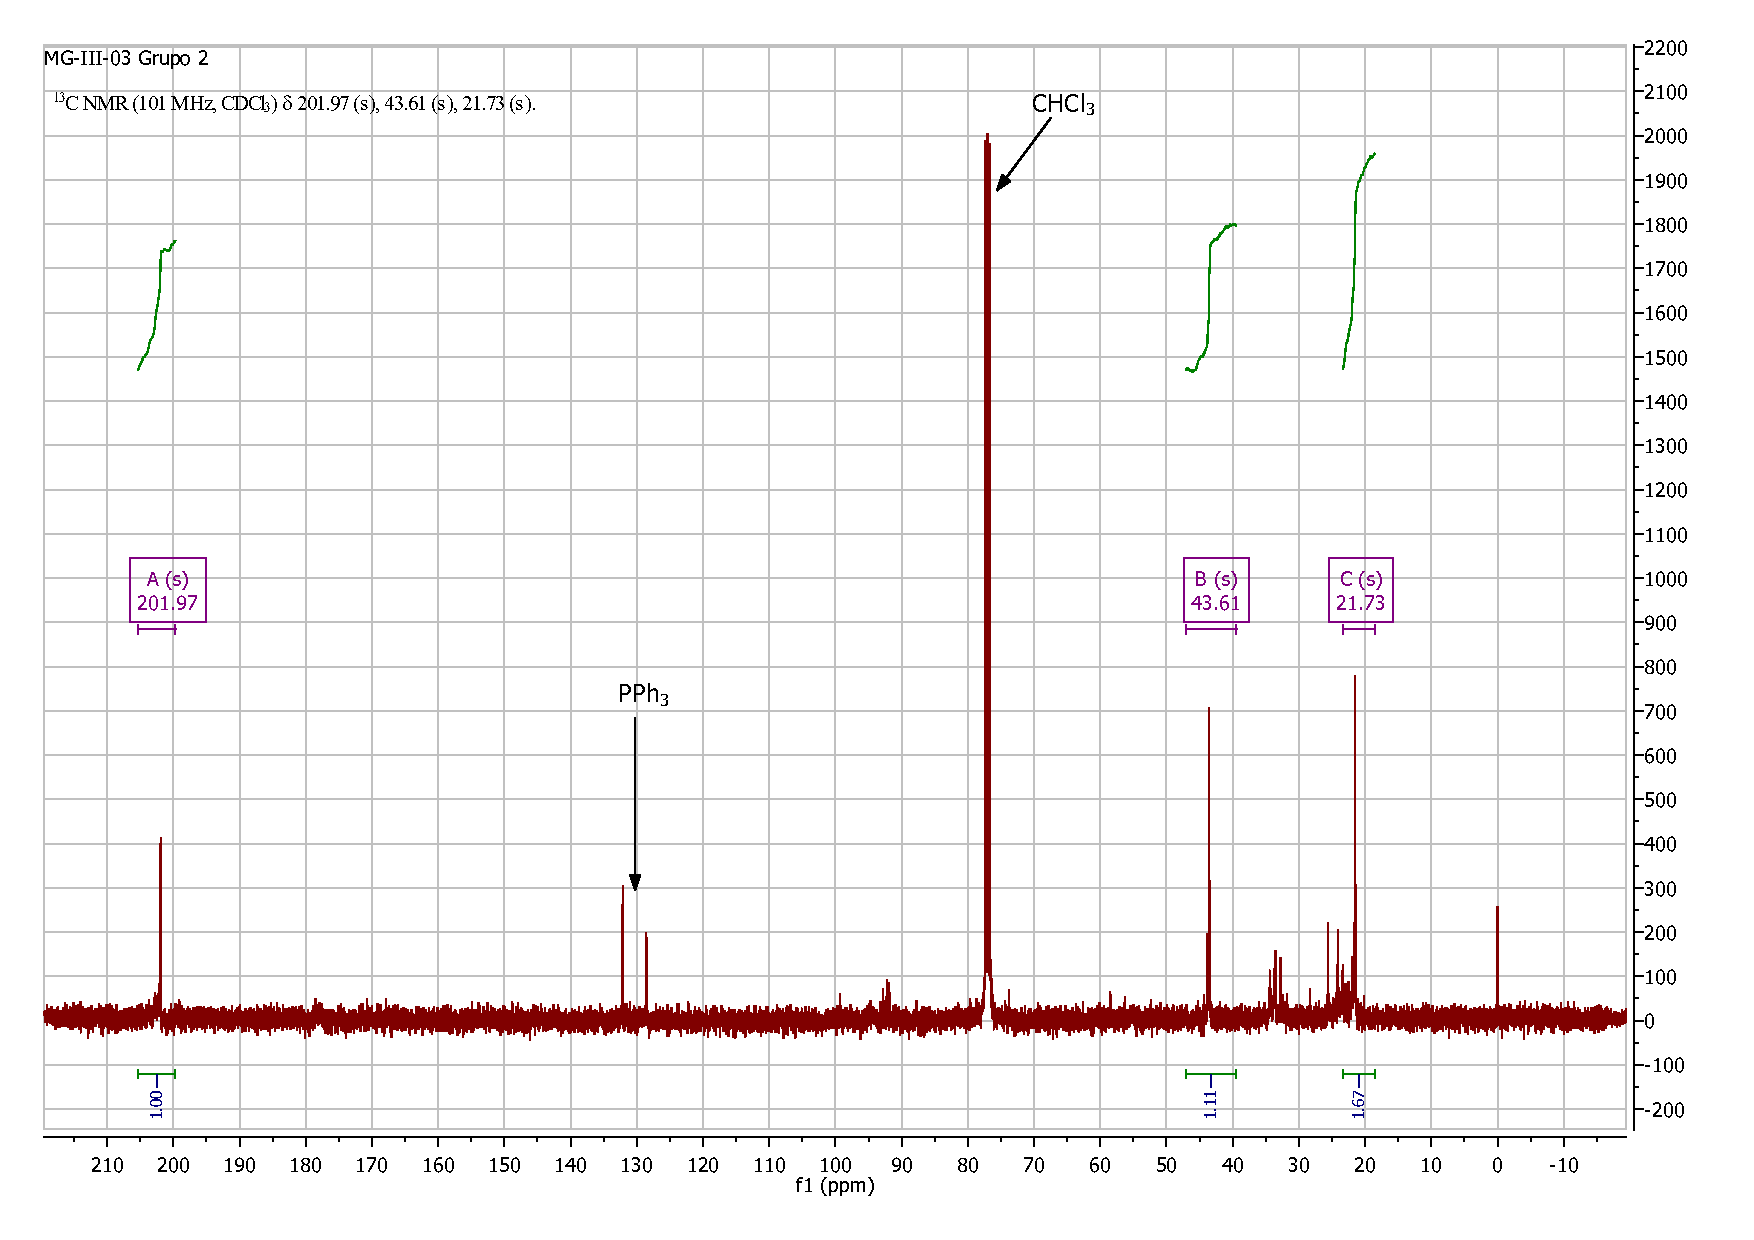
\includegraphics[width=0.5\textheight]{RMN/C.pdf}
	\caption{$^{13}$CRMN del producto purificado.}
\end{figure}
\end{document}